\documentclass{standalone}
\makeatletter\AtBeginDocument{\@buildstepset{1,2,3,4,5}}\makeatother
\usepackage{tikz}
\usetikzlibrary{intersections, calc}
\usepackage{hsbcommon}
    \begin{document}
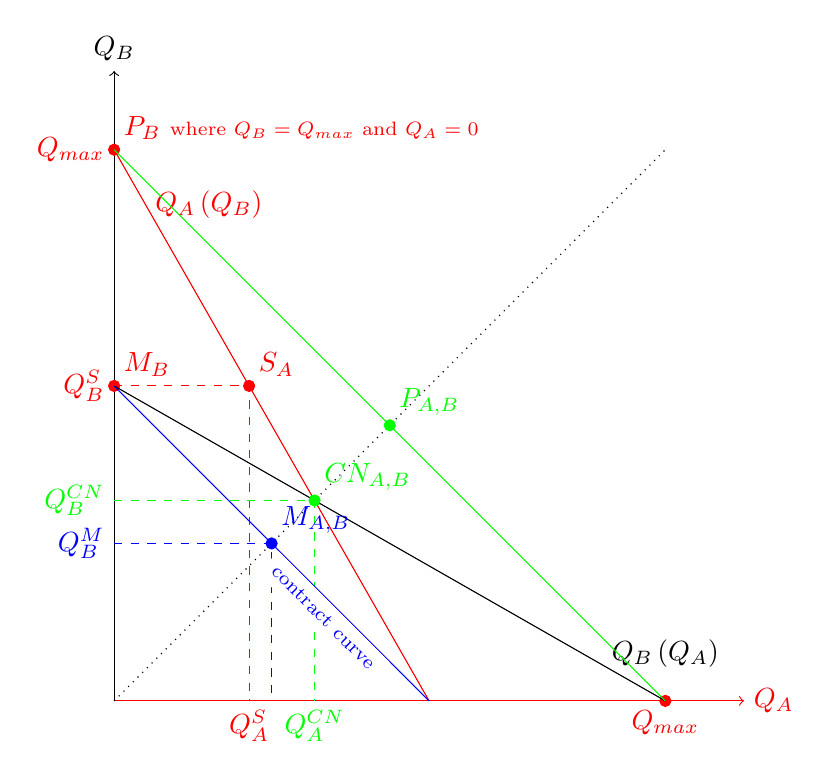
\begin{tikzpicture}
           
        \draw[->,red] (0,0) node[below] {\phantom{$X_i$}} -- (8,0) node[right] (Q) {$Q_A$};
        \draw[->] (0,0) node[left] {\phantom{$Y_mi$}} -- (0,8) node[above] (P) {$Q_B$};


        \coordinate (A) at (0,7);
        \coordinate (B) at (4,0);

        \draw[dotted] (0,0) -- (7,7);

        
        \coordinate (C) at (0,4);
        \coordinate (D) at (7,0);
        \path[name path=responsea] (A) -- (B);
        \path [name path=responseb]  (C) -- (D) ;
        
        \ifstep{2}{
            \begin{scope}[red]
            \filldraw (A) node[left] {$Q_{max}$} node[above right] {$P_B$ \scriptsize  where $Q_B=Q_{max} $ and $ Q_A=0$} circle (2pt);
            \draw  (A) -- (B);
            \node[right] at ($(A)!0.1!(B)$) {$Q_A\left(Q_B\right)$};
            \filldraw (C) node[above right] {$M_B$} circle (2pt);
            \filldraw (D) node[below] {$Q_{max}$}  circle (2pt);
            \end{scope}    
            
            \draw   (C) -- (D) ;
            \node[above=2ex] at (D) {$Q_B\left(Q_A\right)$};
        }
        
        \coordinate (Y) at (B|-, |-C); %% hilfspunkt.  malen nach zahlen.

        \ifstep{1}{%%% price taking equilibrium
            \begin{scope}[green]
                \draw (A) -- (D);
                \coordinate (PP) at ($(A)!0.5!(D)$);
                \filldraw (PP) node[above right] {$P_{A,B}$} circle (2pt);
                \coordinate (PQ) at ($(A)!0.2!(D)$);
                % \node[above right] at  ($(A)!0.3!(D)$) {\scriptsize market capacity};
            \end{scope}
        }

        \ifstep{3}{ %%% stackelberg
            \begin{scope}[red]

            % \filldraw (Y) node[above right] {$P$} circle (2pt);
            \path[name path=stackel] (Y |- ,0) -- (Y) -- (0, |- Y);            
            \path[name intersections={of=stackel and responsea}];
            \filldraw (intersection-2) node[above right] {$S_A$} circle (2pt);
            
            \draw[dashed,name path=stackin1] (0,|- intersection-2) node[left] {$Q^S_B$} -- (intersection-2) --(intersection-2 |-,0) node[below] {$Q^S_A$};    
    
            % \path[name intersections={of=stackel and responseb}];
            % \filldraw (intersection-1) node[above right] {$S_B$} circle (2pt);
            
            % \draw[dashed,name path=stackin2] (0,|- intersection-1)  -- (intersection-1) --(intersection-1 |-,0) ;
            
            % \path[name intersections={of=stackin1 and stackin2,by=inner}]; 
            % \filldraw (inner) node[below left] {$C$} circle (2pt);
                
            \end{scope}
        }

        \ifstep{4}{
        \begin{scope}[green]            
            \path [name intersections={of=responsea and responseb,by=O}];
            \filldraw (O) node[above right] {$CN_{A,B}$} circle (2pt);
    
            \draw[dashed] (0,|-O) node[left] {$Q^{CN}_B$} -- (O) -- (O|-,0) node[below] {$Q^{CN}_A$};
        \end{scope}
        
        }

        \ifstep{5}{
        \begin{scope}[color=blue]
            \draw [name path=cartel] (B) -- (C);
            \coordinate (K) at ($(B)!0.5!(C)$);  %% punkt in der mitte
            \filldraw (K) node[above right] {$M_{A,B}$} circle (2pt);
            \draw[dashed] (0,|-K) node[left] {$Q^M_B$} -- (K) -- (K|-,0);
            \node[below,fill=white,rotate=-45] at ($(B)!0.3!(C)$) {\scriptsize contract curve};  %% punkt in der mitte
        \end{scope}
}

        
        
    \end{tikzpicture}
\end{document}
